\documentclass[a4paper,12pt,twoside]{report}
\usepackage[utf8]{inputenc}
\usepackage{pdflscape}

% Language & Encoding
\usepackage[T1]{fontenc}
\usepackage[german]{babel}  % Deutsche Sprache in automatisch generiertem
\usepackage[fixlanguage]{babelbib}
\usepackage[utf8]{inputenc}

% General Setup
\usepackage{etex}
\usepackage{ifthen}     % If-Then-Statements
\usepackage{pdfpages}
\usepackage{tikz}
\usetikzlibrary{shapes,arrows,topaths,automata}

\definecolor{Blue}{HTML}{2D2F92}
\definecolor{OliveGreen}{HTML}{3C8031}
\definecolor{Fuchsia}{HTML}{8C368C}

\author{Chris Köcher, Philipp Schlag}
\title{Projektseminar: Experimentelle Untersuchung des ``Split-and-Share''-Verfahrens}
\date{Wintersemester 2015/2016\\\small Letzte Änderung: \today}

\usepackage{hyperref}      % Hyperlinks & PDF specific information
\hypersetup{
 unicode,
 hypertexnames=false,
 linkcolor=Blue,
 citecolor=OliveGreen,
 urlcolor=Fuchsia,
 colorlinks=true,
 linktoc=all,
 pdfborder={0 0 0},
 pdftitle={Projektseminar: Experimentelle Untersuchung des "Split-and-Share"-Verfahrens},
 pdfauthor={Chris Köcher, Philipp Schlag}
}

% Page Geometry
\usepackage[a4paper]{geometry}  % A4-Seite mit vielen Layout-Optionen
\geometry{
    twoside
}

\evensidemargin0.5cm
\oddsidemargin0.5cm
%\addtolength{\textwidth}{0cm}
%\setlength{\headheight}{13pt}
\addtolength{\voffset}{0.75cm}
%\addtolength{\textheight}{1.5cm}

%\parindent 0pt

% Fonts & Symbols
\usepackage{latexsym}       % Fuer recht seltene Zeichen
\usepackage{amsfonts}       % Mathe-Schriften
\usepackage{amssymb}        % Symbole
\usepackage{amsmath}        % Symbole
\usepackage{lmodern}        % verwenden der "Latin Modern" ("Computer Modern"++)

\newcommand{\origttfamily}{}    % Trenner für Typewriter
\let\origttfamily=\ttfamily
\renewcommand{\ttfamily}{\origttfamily \hyphenchar\font=`\-}


%
% Document Layout

\usepackage[activate]{pdfcprot} % Margin-Kerning für ein besseres Gesamtbild

% Header & Footer
\usepackage{fancyhdr}       % Kopfzeilen formatieren
\pagestyle{fancy}
\fancyhf{}
\setlength{\headheight}{15pt}
\fancyhead[LE,RO]{\thepage}
\fancyhead[RE]{\scshape \nouppercase{\leftmark}}
\fancyhead[LO]{\scshape \nouppercase{\rightmark}}
\renewcommand{\headrulewidth}{0.4pt}
\renewcommand{\footrulewidth}{0.4pt}
\fancypagestyle{plain}{
 \fancyhead[RE,LO]{}
 \renewcommand{\headrulewidth}{0pt}
}
\fancypagestyle{simple}{
 \fancyhead[RE,LO]{}
 \renewcommand{\headrulewidth}{0pt}
 \renewcommand{\footrulewidth}{0pt}
}
\fancypagestyle{light}{
 \fancyhead[RE,LO]{}
}

% ClearDoublePage fix
\makeatletter 
\def\cleardoublepage{\clearpage\if@twoside \ifodd\c@page\else% 
%\hbox{}% 
%\thispagestyle{simple}
%\newpage% 
%\if@twocolumn\hbox{}\newpage\fi
\fi\fi}
\makeatother 

% Headlines
\renewcommand{\thechapter}{\Roman{chapter}}
\newcounter{newchapter}
\numberwithin{section}{newchapter}
\renewcommand{\thefigure}{\arabic{chapter}.\arabic{figure}}
\renewcommand{\thetable}{\arabic{chapter}.\arabic{table}}
%\renewcommand{\thesection}{\arabic{chapter}.\arabic{section}}

\usepackage{titlesec}
\setcounter{secnumdepth}{3}
\titleformat{\chapter}[display]%
    {\huge\center\bf}%
    {\Large\mdseries\scshape Kapitel \thechapter}%
    {0cm}{\setcounter{newchapter}{\value{chapter}}}[\vspace{2ex}\titlerule]
\titlespacing*{\chapter}{0pt}{0ex}{8ex}
\titleformat{\subsubsection}{\normalsize\bfseries}{\thesubsubsection}{.75em}{}
\titleformat{\paragraph}[runin]{\bfseries}{}{0pt}{}[.]
\titleformat{\subparagraph}[runin]{\itshape}{}{0pt}{}[.]

% Table of Contents
\usepackage[titles]{tocloft}

\setlength{\cftbeforetoctitleskip}{0ex}
\setlength{\cftaftertoctitleskip}{0ex}
\renewcommand{\cfttoctitlefont}{}

\setlength{\cftbeforeloftitleskip}{4ex}
\setlength{\cftafterloftitleskip}{1ex}
\renewcommand{\cftloftitlefont}{\LARGE}

\setlength{\cftbeforelottitleskip}{4ex}
\setlength{\cftafterlottitleskip}{1ex}
\renewcommand{\cftlottitlefont}{\LARGE}

\newcommand\listingname{Verzeichnis der Listings}
\newlistof[chapter]{listing}{lst}{\listingname}
\setlength{\cftbeforelsttitleskip}{4ex}
\setlength{\cftafterlsttitleskip}{1ex}
\renewcommand{\cftlsttitlefont}{\LARGE}

\newcommand\theoremsname{Theoremverzeichnis}
\newlistof[chapter]{theorems}{lthm}{\theoremsname}
\setlength{\cftbeforelthmtitleskip}{4ex}
\setlength{\cftafterlthmtitleskip}{1ex}
\renewcommand{\cftlthmtitlefont}{\LARGE}

\setcounter{tocdepth}{2}
\setlength{\cftbeforechapskip}{1.0ex}
\setlength{\cftbeforesecskip}{0ex}
\setlength{\cftbeforesubsecskip}{-.2ex}
\newcommand\tocentry[1]{\addcontentsline{toc}{chapter}{#1}}
\newcommand{\ttsubsection}[1]{\subsection[\texorpdfstring{\texttt{\slshape #1}}{#1}]{\texttt{#1}}}
\newcommand\addtotheorems[2]{
    \refstepcounter{theorems}
    \addcontentsline{lthm}{theorems}{\protect\numberline{\thetheorems}\textbf{#1:} #2}
}
\newcommand\addlistspace[1]{
    \addtocontents{#1}{\vspace{1.3ex}}
}
\setlength{\cftchapnumwidth}{20pt}
\setlength{\cftsecnumwidth}{20pt}
\setlength{\cftsecindent}{20pt}
\setlength{\cftsubsecindent}{40pt}

% Glossar
%\usepackage[number=none,style=altlist]{glossary}
%\renewcommand{\glosslabel}[2]{\sffamily #2}
%\makeglossary


%
% Page Elements

% Captions & Figures
\usepackage{graphicx}       % Grafiken einbinden mit vielen Optionen
\graphicspath{{./figures/}}

% Tables
\usepackage{booktabs}       % Bessere Tabellen.

% Theorems
\usepackage{framed}     % Rahmen für Theoreme
\usepackage{soul}
\usepackage[amsmath,framed,thmmarks,standard]{ntheorem} % erweiterte Theorem-Umgebungen.
\newcounter{main}[chapter]
\numberwithin{main}{newchapter}
\newcounter{sub}[main] %beginne mit jedem Theorem von vorn

\makeatletter
 \newtheoremstyle{subtheorem}%
 {\item[\hskip\labelsep \theorem@headerfont \underline{##1\ ##2\theorem@separator}]}%
 {\item[\hskip\labelsep \theorem@headerfont \underline{##1\ ##2\ (##3)\theorem@separator}]}%
 \newtheoremstyle{subtheoremnonumber}%
 {\item[\theorem@headerfont\hskip\labelsep \underline{##1\theorem@separator}]}%
 {\item[\theorem@headerfont\hskip\labelsep \underline{##1\ (##3)\theorem@separator}]}%
\makeatother

%Theoreme in Kästchen
\theoremseparator{.}
\theorembodyfont{\itshape}
\theoremindent 6pt
\newframedtheorem{fsatz}[main]{Satz}
\newframedtheorem{flemma}[main]{Lemma}
\newframedtheorem{fkorollar}[main]{Korollar}
\newframedtheorem{fproposition}[main]{Proposition}
\newframedtheorem{fbehauptung}[main]{Behauptung}
\renewtheorem{satz}[main]{Satz}
\renewtheorem{lemma}[main]{Lemma}
\renewtheorem{korollar}[main]{Korollar}
\renewtheorem{proposition}[main]{Proposition}
\newframedtheorem{behauptung}[main]{Behauptung}
\newframedtheorem{fakt}[main]{Fakt}

%Theoreme ohne Kästchen, eingerückt
\theorempreskip{5pt}
\theorempostskip{5pt}
\theoremindent 15pt
\theorembodyfont{\upshape}
\newtheorem{fdefinition}[main]{Definition}
\renewtheorem{definition}[main]{Definition}
\renewtheorem{beispiel}[main]{Beispiel}
\newtheorem{algo}[main]{Algorithmus}
\newtheorem{fbemerkung}[main]{Bemerkung}
\newtheorem{fbemerkungen}[main]{Bemerkungen}
\newtheorem{falgorithmus}[main]{Algorithmus}
\newtheorem{fbeobachtung}[main]{Beobachtung}

%Sub-Theoreme mit Nummerierung
\theorempreskip{0pt}
\theorempostskip{0pt}
\theoremseparator{.}
\theoremheaderfont{\normalfont\itshape\ul}
\theoremindent 0pt
\theoremstyle{subtheorem}
\newtheorem{subbehauptung}[sub]{Behauptung}
\newtheorem{subbeobachtung}[sub]{Beobachtung}

%Sub-Theoreme ohne Nummerierung
\theoremstyle{subtheoremnonumber}
\newtheorem{subanmerkung}{Anmerkung}
\newtheorem{subidee}{Idee}
\renewtheorem{subbehauptung*}{Behauptung}
\newtheorem{subbeispiel}{Beispiel}
\theoremsymbol{\ensuremath{_{\operatorname{q.e.d.}}}}
\newtheorem{subbeweis}{Beweis}

%Theoreme mit Einrückung, ohne Kästchen, ohne Nummerierung
\theorempreskip{5pt}
\theorempostskip{5pt}
\theoremseparator{.\setcounter{sub}{0}}
\theoremheaderfont{\normalfont\bfseries}
\theoremsymbol{}
\theoremstyle{nonumberplain}
\theoremindent 15pt
\renewtheorem{bemerkung}{Bemerkung}
\renewtheorem{beispiel*}{Beispiel}
\renewtheorem{falgorithmus*}{Algorithmus}
\renewtheorem{fbeobachtung*}[main]{Beobachtung}

%Theoreme ohne Einrückung, ohne Kästchen, ohne Nummerierung
\theoremindent 0pt
\theoremsymbol{\ensuremath{_\blacksquare}}
\renewtheorem{beweis}{Beweis}
\newtheorem{beweisidee}{Beweisidee}
\newtheorem{beweisstrategie}{Beweisstrategie}

\theorembodyfont{\itshape}
\theoremsymbol{}
\renewtheorem{satz*}{Satz}


%
% Inline

\usepackage{url}        % URL's zitieren
\usepackage{numprint}       % Zahlen formatieren
\newcommand\notice[1]{}     % Notiz
\newcommand\seppar{ \vspace{2ex} \noindent } % Neuer Absatz
\newcommand\name[1]{{\em #1}}   % Namen
%\newcommand\ilcapt[1]{{\sffamily\bfseries #1}} % inline caption

\usepackage[german]{todonotes}
\usepackage{enumitem}

\setlist[enumerate]{label=(\roman*)}
\numberwithin{equation}{newchapter}

\usepackage{float}
\usepackage[hypcap,labelsep=period,labelfont=bf]{caption}


% Listings
\usepackage{minted}
\usepackage[plain,longend,linesnumbered]{algorithm2e}

\makeatletter
\renewcommand{\@algocf@capt@plain}{top}
\renewcommand{\algocf@makecaption@plain}[2]{%
  \global\sbox\algocf@capbox{\hskip\AlCapHSkip% .5\algomargin%
    \parbox[t]{\hsize}{\algocf@captiontext{#1}{#2}}}% then caption is not centered
}
\makeatother

\newlength{\algoindent}
\setlength\algoindent{15pt}

\newcommand{\capsty}[1]{\underline{\FuncSty{#1}}}
\SetKwInput{KwIn}{Eingabe}
\DontPrintSemicolon
\SetAlgoLined
\SetNlSty{textnormal}{(}{)}
\SetAlgoNlRelativeSize{-3}
\SetAlgorithmName{}{}{}
\SetAlCapNameSty{capsty}
\SetAlgoCaptionSeparator{}
\SetAlCapSkip{0pt}
\SetAlCapHSkip{0pt}
\SetAlgoInsideSkip{noskip}
\NoCaptionOfAlgo


%Weiteres Zeugs....
\newcommand{\IA}{\textup{(IA)}\xspace}
\newcommand{\IV}{\textup{(IV)}\xspace}
\newcommand{\IS}{\textup{(IS)}\xspace}

\newcommand{\Var}{\operatorname{Var}\nolimits}
\newcommand{\E}{\operatorname{E}\nolimits}
\renewcommand{\Pr}{\operatorname{Pr}\nolimits}
\renewcommand{\O}[1]{\mathcal{O}(#1)}
\newcommand{\bigO}[1]{\mathcal{O}\!\left(#1\right)}

\renewcommand{\mod}{\operatorname{mod}}
\renewcommand{\div}{\operatorname{div}}
\newcommand{\GF}{\operatorname{GF}}
\newcommand{\id}{\operatorname{id}}

%Noch mehr weiteres Zeugs...
\usepackage{changepage}
\usepackage{chngcntr}
\usepackage{afterpage}

\newenvironment{problem}[1][15pt]{\begin{adjustwidth}{#1}{0pt}}{\end{adjustwidth}}

\counterwithout{footnote}{chapter}
%\newboolean{myfnonpage}
%\setboolean{myfnonpage}{false}

\fancypagestyle{footnotepage}{
 \renewcommand{\footrulewidth}{0pt}
}

\fancypagestyle{footnotepageplain}{
  \fancyhead[RE,LO]{}
 \renewcommand{\footrulewidth}{0pt}
 \renewcommand{\headrulewidth}{0pt}
}

\newcommand{\myfootnote}[1]{%
\footnote{#1}%
\thispagestyle{footnotepage}%
\enlargethispage{35.7pt}%
}

\newcommand{\myfootnotetext}[1]{%
\footnotetext{#1}%
\thispagestyle{footnotepage}%
\enlargethispage{35.7pt}%
}

\newcommand{\myfootnoteplain}[1]{%
\footnote{#1}%
\thispagestyle{footnotepageplain}%
\enlargethispage{35.7pt}%
}

\newcommand{\myfootnotetextplain}[1]{%
\footnotetext{#1}%
\thispagestyle{footnotepageplain}%
\enlargethispage{35.7pt}%
}

\newcommand{\myfootnotemulti}[1]{%
\footnote{#1}%
\enlargethispage{21.7pt}%
}

\renewcommand{\footnoterule}{%
%\setboolean{myfnonpage}{false}%
\vfill%
\kern 3pt%
\hrule width \textwidth%
\kern 2.6pt%
}

\usepackage{array}
\newcolumntype{x}[1]{>{\centering\arraybackslash\hspace{0pt}}m{#1}}

\usepackage{svg}

\begin{document}
%Titelblatt
\begin{titlepage}

\newcommand{\HRule}{\rule{\linewidth}{0.4pt}} % Defines a new command for the horizontal lines, change thickness here

\center % Center everything on the page
 
%----------------------------------------------------------------------------------------
%   HEADING SECTIONS
%----------------------------------------------------------------------------------------

\
\vspace{3.5cm}

%\textsc{\LARGE University Name}\\[1.5cm] % Name of your university/college
%\textsc{\Large Major Heading}\\[0.5cm] % Major heading such as course name
%\textsc{\large Minor Heading}\\[0.5cm] % Minor heading such as course title

%----------------------------------------------------------------------------------------
%   TITLE SECTION
%----------------------------------------------------------------------------------------

\begin{framed}
 \vspace{0.4cm}
 \Huge \textsc{Projektseminar}\\[0.2cm]
 \normalsize Experimentelle Untersuchung des ``Split-and-Share''-Verfahrens
 \vspace{0.4cm}
\end{framed}


%----------------------------------------------------------------------------------------
%   AUTHOR SECTION
%----------------------------------------------------------------------------------------

\begin{center}
 \large Chris Köcher\qquad\qquad Philipp Schlag\\[3cm]
\end{center}

%----------------------------------------------------------------------------------------
%   DATE SECTION
%----------------------------------------------------------------------------------------

{\large Wintersemester 2015\\\small Letzte Änderung: \today}\\[3cm] % Date, change the \today to a set date if you want to be precise

%----------------------------------------------------------------------------------------
%   LOGO SECTION
%----------------------------------------------------------------------------------------


\includegraphics{logo-tu-ilmenau}\\[1cm] % Include a department/university logo - this will require the graphicx package
 
%----------------------------------------------------------------------------------------

\vfill % Fill the rest of the page with whitespace

\end{titlepage}

\thispagestyle{empty}
\newpage
 
%Inhaltsverzeichnis
\pagenumbering{roman}
\tableofcontents
\newpage
\pagenumbering{arabic}

\newcommand{\size}[1]{\ensuremath{\operatorname{size}_{\operatorname{#1}}}}

\chapter{Konstruktionsverfahren}
\label{cha:konstruktion}

In dieser Arbeit untersuchen wir das ``Split-and-Share''-Verfahren als mögliche Realisierung perfekter Hashfunktionen experimentell. Zunächst möchten wir in diesem Kapitel die von uns verwendeten Algorithmen zur Konstruktion dieser Hashfunktionen beschreiben.
Im Allgemeinen basieren diese auf den in \cite{Dietzfelbinger2007} und \cite{Botelho2013108} dargestellten Methoden und theoretischen Betrachtungen.

\section{Überblick}
\label{sec:ueberblick}

Für eine gegebene Menge $S\subseteq U=\{0, 1\}^{64}$ von 64-Bit-Schlüsseln konstruieren wir unter Verwendung des ``Split-and-Share''-Verfahrens eine perfekte Hashfunktion in Form einer Datenstruktur \texttt{PerfectHashFunction}, die anschließend genutzt werden kann, um für jeden Schlüssel $x\in S$ mittels der Methode \texttt{evaluate} den eineindeutigen Hashwert $h_{\text{perf}}(x)$ zu berechnen.

Das in der Programmiersprache C++ implementierte Kommandozeilen-Pro\-gramm für Linux \texttt{Hashing} (für den Quellcode siehe beigefügte CD oder\linebreak \url{https://github.com/ckoecher/Hashing}) wird dabei in der Form
\begin{center}
 \texttt{./Hashing <configuration file> <data file> <statistics file>}
\end{center}
aufgerufen.
In der Konfigurationsdatei können diverse Parameter zur Erzeugung der Hashfunktion festgelegt werden.
Dadurch kann z.B. die Anzahl der erzeugten Buckets variiert oder der Startwert des Zufallszahlengenerators gesetzt werden.
Aus der Datendatei werden die Schlüssel als 64-Bit-Einheiten im Binärmodus gelesen.
Zum Schluss werden statistische Kenngrößen der Konstruktion, z.B. die benötigten Zeiten der einzelnen Konstruktionsphasen, der Speicherplatz der erzeugten Datenstruktur und die Anzahl wiederholter Versuche, in der Statistikdatei gespeichert.

Im Folgenden verwenden wir Standardwerte, wie sie in \cite{Dietzfelbinger2007} und \cite{Botelho2013108} beschrieben werden.

\section{Erzeugung von Zufallszahlen}
\label{sec:zufallszahlen}

Als Zufallszahlengenerator zur Erzeugung der notwendigen (Pseudo-)Zufallszahlen, natürliche Zahlen innerhalb variierender Wertebereiche, verwenden wir die in der C++-Standardbibliothek (seit C++11) enthaltene Implementierung \texttt{mt19937} des Mersenne-Twisters.

\section{1-universelle Hashfunktionen}
\label{sec:einsuniverselleHF}

Unsere elementaren Grundbausteine zur Konstruktion der perfekten Hashfunktion sind 1-universelle Hashfunktionen $h\colon U\to [m']=\{0, 1, \dots, m'-1\}$.
Dabei wird jeder Schlüssel $x\in S$ in $l$ Teilschlüssel bestehend aus $k$ Bit aufgeteilt, d.h.\linebreak $x=x_0\dots x_{l-1}$ mit $x_0, \dots, x_{l-1}\in\{0, 1\}^{k}$.

Um eine solche 1-universelle Hashfunktionen zufällig zu wählen, werden $l+1$ Koeffizienten $a_0, a_1, \dots, a_l$ aus $\left[2^{k+\lceil\log m'\rceil+6}\right]$ zufällig gewählt.
Der Hashwert berechnet sich dann wie folgt:
\[h(x)=h(x_0\dots x_{l-1})=\underbrace{\left(\left(\left(a_l+\sum\limits_{i=0}^{l-1}{a_i x_i}\right)\mod 2^{k+\lceil\log m'\rceil+6}\right)\div 2^k\right)}_{=h'(x)}\mod m'.\]
Da der innere Teil der Funktion (alles bis auf $\mod m'$) eine 2-fach unabhängige Hashfunktion $h'\colon U\to [2^{\lceil\log m'\rceil+6}]\approx[m'\cdot 2^6]$ ist, ist $h$ selbst (annähernd) 1-universell.

\section{Split in kleine Buckets}
Zur Wahl einer geeigneten Anzahl von Buckets $m$, die von der zufällig gewählten Split-Funktion erzeugt werden, haben wir zwei mögliche Verfahren implementiert, welche im Folgenden kurz erläutert werden sollen.

\subsection{Parametrisiertes Verfahren}
\label{sec:splitParametrisiert}

Zunächst werden die $n=|S|$ 64-Bit-Schlüssel in $m=\min\left\{\lceil 2 n^{2/3}\rceil, \lceil\frac{n}{20}\rceil\right\}$ Buckets aufgeteilt.
Sowohl der Koeffizient als auch der Exponent zur Bestimmung der Anzahl von Buckets sind dabei durch Konfigurationsparameter variierbar.
(In diesen beiden liegt auch besonders viel Potenzial für eine Verbesserung in der Konstruktion bzgl. Konstruktionsdauer und Größe der erzeugten Datenstruktur.)
Die zusätzliche Einschränkung, dass höchstens $\lceil\frac{n}{20}\rceil$ Buckets erzeugt werden, soll für kleine $n$ die Wahrscheinlichkeit verringern, dass zu viele zu kleine Buckets entstehen.

\pagebreak

In der Split-Phase werden sämtliche Schlüssel aus der Datendatei mehrfach eingelesen.
Zunächst wird für die zufällig gewählte 1-universelle Hashfunktion $h_{\text{split}}\colon U\to [m]$ getestet, ob alle $m$ Buckets höchstens $\max\left\{\lfloor\sqrt{n}\rfloor, 40\right\}$ Schlüssel enthalten, d.h. nicht zu groß werden (Counting).
Für $i\in[m]$ bezeichne $n_i$ die Anzahl der Schlüssel, die in Bucket $i$ enthalten sind.
Dann ist $\hat{n}=\max\{n_i\,|\,i\in[m]\}$ die maximale Bucketgröße und nach \cite[Lemma 1]{Dietzfelbinger2007} gilt $\Pr\left(\hat{n}\le\sqrt{n}\right)\ge\frac{3}{4}$.
Im positiven Fall werden die Schlüssel noch einmal eingelesen und in einer temporären Datei derart gespeichert, dass alle Schlüssel desselben Buckets direkt hintereinander in der Datei stehen (Splitting)\myfootnote{Wir haben uns für diese zeitintensivere Variante entschieden, damit auch für größere Schlüsselmengen das Konstruktionsverfahren noch auf einem gewöhnlichen PC ohne übermäßig viel Arbeitsspeicher ausgeführt werden kann.}.

Im weiteren Verlauf wird für jeden Bucket $i$ eine perfekte Hashfunktion mit Wertebereich $[m_i]$ konstruiert, wobei $m_i=\lceil1,25\cdot n_i\rceil$ ist. (Auch der Koeffizient $1,25$ kann in der Konfigurationsdatei variiert werden.)
Allerdings muss zusätzlich sichergestellt werden (ggf. durch einfache Vergrößerung), dass $m_i\ge 10$ gilt, falls $m_i>0$ ist.
Das Konstruktionsverfahren alleine benötigt $m_i\ge 3$, da als Zwischenschritt für jeden Schlüssel des Buckets $i$ drei verschiedene Hashwerte in $[m_i]$ berechnet werden müssen.
Um weitere Schwierigkeiten bei der Erzeugung der perfekten Hashfunktion für Bucket $i$ mit besonders wenigen Schlüsseln (in Tests war dies besonders für $2\le n_i\le 5$ der Fall, weil dann $m_i$ mit $3\le m_i\le 7$ zu klein ist) zu vermeiden, hat sich $m_i\ge 10$ als ausreichender Wert herausgestellt.

\subsection{Automatisiertes Verfahren}
\label{sec:splitAutomatisiert}

Werden die Parameter derart gewählt, dass für die Anzahl zu erzeugender Buckets $m=0$ gelten würde, so wird im Programm eine Anzahl von Buckets berechnet, die den Gesamtspeicherplatz der am Ende erzeugten Datenstruktur zu minimieren versucht.
Dieser ist im Wesentlichen von der Anzahl der Buckets $m$ und der maximalen Bucketgröße $\hat{n}$ abhängig.
Basierend auf \cite[Theorem 1]{Raab1998} und experimenteller Untersuchungen, die in Abschnitt \ref{sec:schaetzungBucketgroesse} erläutert werden, hat sich gezeigt, dass \[\frac{n}{m}+\sqrt{\frac{2\cdot n\cdot\log m}{m}}\] eine sinnvolle Abschätzung für $\hat{n}$ darstellt.
Mit dieser ist es möglich, diejenige Anzahl von Buckets $m$ zu bestimmen, sodass der Gesamtspeicherplatz (unter der Annahme, dass $\hat{n}$ tatsächlich den Wert der Abschätzung annimmt) minimiert wird.

\section{Geteilte Datenstruktur}
\label{sec:geteilteDatenstruktur}

Um für jeden einzelnen Bucket eine perfekte Hashfunktion zu konstruieren, werden insbesondere sechs Tabellen $T_0^0, T_0^1, T_0^2, T_1^0, T_1^1, T_1^2$ gemeinsam genutzt.
Jede Tabelle enthält $r=\lceil 2 \hat{n}^{3/2}\rceil$ Einträge zufälliger Bitzahlen der Länge $b=\lceil\log\hat{n}\rceil+6$.
Um die Versagenswahrscheinlichkeit weiter zu minimieren, wird für jeden Bucket $i$ noch eine weitere zufällige Bitzahl $s_i\in[2^b]$ genutzt.
Indem einzelne $s_i$ oder sämtliche Tabellen mit neuen zufälligen Zahlen gefüllt werden, können die folgenden Konstruktionsschritte im Falle eines Versagens wiederholt werden. Die maximale Anzahl solcher Wiederholungen kann in der Konfigurationsdatei angegeben werden.

\section[Gute Paare 1-universeller Hashfunktionen pro Bucket]{Gute Paare 1-universeller Hashfunktionen\linebreak pro Bucket}
\label{sec:gutePaare}

Für jeden Bucket $i\in[m]$ mit Schlüsselmenge $S_i$ wird zunächst ein gutes Paar $(h_0^i, h_1^i)$ 1-universeller Hashfunktionen $h_0^i, h_1^i\colon U\to[r]$ zur Ansteuerung der Tabelleneinträge erzeugt.
Dabei heißt das Paar $(h_0^i, h_1^i)$ \textbf{gut}, wenn für jeden Schlüssel $x\in S_i$ einer der Hashwerte eineindeutig ist, d.h. es gibt ein $j\in\{0, 1\}$ derart, dass $h_j^i(x)\neq h_j^i(y)$ für alle $y\in S_i\setminus\{x\}$ gilt.
Nach \cite[Lemma 2]{Dietzfelbinger2007} gilt $\Pr\left((h_0^i, h_1^i)\text{ ist gut}\right)\ge\frac{3}{4}$.

\section{Uniforme Hashfunktionen pro Bucket}
\label{sec:uniformeHashfunktionen}

Ist $(h_0^i, h_1^i)$ ein gutes Paar 1-universeller Hashfunktionen, so sind die Funktionen $f_0^i\colon U\to[m_i]$, $f_1^i\colon U\to[m_i-1]$ und $f_2^i\colon U\to[m_i-2]$ mit \[\begin{array}{l}f_0^i(x)=\left(T_0^0[h_0^i(x)]\cdot s_i\oplus T_1^0[h_1^i(x)]\right)\mod m_i\\f_1^i(x)=\left(T_0^1[h_0^i(x)]\cdot s_i\oplus T_1^1[h_1^i(x)]\right)\mod (m_i-1)\\f_2^i(x)=\left(T_0^2[h_0^i(x)]\cdot s_i\oplus T_1^2[h_1^i(x)]\right)\mod (m_i-2)\end{array}\] für $x\in S_i$ rein zufällig auf ihren jeweiligen Wertebereichen.
Dabei beschreibt $\oplus$ das bitweise XOR (auf Bitzahlen der Länge $b$).

Daraus können leicht drei Funktion $g_0^i, g_1^i, g_2^i\colon U\to [m_i]$ konstruiert werden, wobei die Menge $\{g_0^i(x), g_1^i(x), g_2^i(x)\}$ eine rein zufällige dreielementige Teilmenge von $[m_i]$ ist.

\section{Perfekte Hashfunktionen pro Bucket}
\label{sec:perfekteHashfunktionProBucket}

Damit können wir für jeden Bucket $i\in[m]$ einen 3-Graphen $G_3^i=(V, E)$ konstruieren mit \[\begin{array}{l}V=[m_i]\text{ und}\\E=\left\{\,\{g_0^i(x), g_1^i(x), g_2^i(x)\}{\;\ifnum\currentgrouptype=16 \middle\fi\mid\;}x\in S_i\,\right\}.\end{array}\]
Es gilt:
\[\begin{array}{cl}
&G_3^i\text{ ist azyklisch.}\\
\Leftrightarrow&\text{Aus }G_3^i\text{ können durch wiederholtes Löschen von Kanten mit inzidenten}\\
&\text{Knoten vom Grad }1\text{ alle Kanten entfernt werden.}\\
\Rightarrow&\text{Jeder Kante }e\in E\text{ kann eineindeutig eine inzidente Ecke zugeordnet werden.}\\
\Leftrightarrow&\text{Jedem Schlüssel }x\in S_i\text{ kann eineindeutig ein Hashwert }h\in[m_i]\\
&\text{zugeordnet werden, wobei }h\in\{g_0^i(x), g_1^i(x), g_2^i(x)\}.\\
\Rightarrow&\text{Es gibt eine perfekte Hashfunktion }h_i\colon U\to[m_i]\text{ für }S_i,\text{ die ``leicht'' aus }G_3^i\\
&\text{berechnet werden kann.}
\end{array}\]
Für die Berechnung dieser perfekten Hashfunktion wird wie in \cite[Theorem 6.4]{czech1997} beschrieben eine Funktion $g_i\colon[m_i]\to\{0, 1, 2\}$ aus $G_3^i$ konstruiert, mit deren Hilfe schließlich der passende Hashwert $h_i(x)\in\{g_0^i(x), g_1^i(x), g_2^i(x)\}$ für $x\in S_i$ bestimmt werden kann.

Nach \cite[Theorem 3.5]{Botelho2013108} gilt
\[\lim_{m_i\to\infty}{\Pr(G_3^i\text{ ist azyklisch})}=1.\]
Tatsächlich haben unsere Tests mit rein zufälligen Schlüsselmengen untermauert, dass die Wahrscheinlichkeit auch für kleinere $m_i$ zufriedenstellend ist.

\section{Berechnung des Hashwertes}
\label{sec:berechnungHashwert}

Sei $x\in S$ beliebig.
Dann gehört $x$ zum Bucket $i=h_{\text{split}}(x)$.
Der Offset des Wertebereiches $[m_i]$ dieses Buckets im Gesamtwertebereich ist dann
\[\operatorname{offset}_i=\sum_{j=0}^{i-1}{m_j}.\]
Aus den drei Werten $g_0^i(x)$, $g_1^i(x)$, und $g_2^i(x)$ wird der Index
\[j=(g_i[g_0^i(x)]+g_i[g_1^i(x)]+g_i[g_2^i(x)])\mod 3\]
bestimmt. Dann berechnet sich der tatsächliche Hashwert von $x$ wie folgt:
\[h_{\text{perf}}(x)=\operatorname{offset}_i+g_j^i(x).\]


\chapter{Untersuchungen und Ergebnisse}
\label{cha:untersuchungenErgebnisse}

\section{Testumgebung}
\label{sec:testumgebung}

Die in den weiteren Abschnitten angegebenen Tests wurden allesamt auf einem Rechner mit folgenden Spezifikationen durchgeführt:
%\begin{itemize}
% \item \emph{Betriebssystem:} Ubuntu Linux 15.10 (Kernel: 4.2)
% \item \emph{Prozessor:} Intel\textregistered Core\texttrademark i7-4702MQ CPU (2.20GHz) mit 6144 KB L2-Cache
% \item \emph{Hauptspeicher:} 7903 MiB
% \item \emph{Compiler:} GCC 5.2.1 mit CMake 3.3.2
%\end{itemize}
\begin{itemize}
 \item \emph{Betriebssystem:} Linux Mint 17.1 Cinnamon 64-bit (Kernel: 3.13)
 \item \emph{Prozessor:} Intel$^{\textregistered}$ Core$\texttrademark$ i7-2600 CPU (3.40GHz) mit 128 kB L1-Cache, 1024 kB L2-Cache, 8192 kB L3-Cache
 \item \emph{Hauptspeicher:} 11.7 GiB
 \item \emph{Compiler:} GCC 4.8.4
\end{itemize}

\section{Ablauf der experimentellen Untersuchungen}
\label{sec:experimentelleUntersuchungen}

Im Folgenden werden die Ergebnisse zu Testläufen mit Schlüsselmengen der Größe $10^4$, $10^5$, $10^6$, $10^7$ und $10^8$ präsentiert, wobei wir uns insbesondere für die letzten drei interessieren.
Pro Größenordnung wurden fünf verschiedene zufällige Schlüsselmengen mit den in der \texttt{config.ini} Datei enthaltenen Parametern untersucht, wobei pro Schlüsselmenge fünf Durchläufe mit jeweils anderem Startwert für den Zufallszahlengenerator durchgeführt wurden.
Konkret wurden die Seeds ``1'', ``42'', ``1337'', ``123456'' und ``9892002'' verwendet. Damit wurden pro Größenordnung jeweils $25$ Testläufe durchgeführt.

Ergänzt werden diese Ergebnisse durch Daten über einen einzelnen Testlauf mit $10^9$ Schlüsseln.
Da ein solcher Durchlauf (insbesondere aufgrund des hohen Zeitaufwandes für das Lesen aus und das Schreiben in Dateien) bereits mehrere Stunden tatsächliche Zeit (nicht nur CPU-Zeit) benötigt, und wir uns im Rahmen der Experimente nur für ``kleine'' Schlüsselmengen interessiert haben, soll dies genügen.

Sämtliche erhobenen Daten (sowohl die hier präsentierten als auch weitere) können in der beigefügten Datei \texttt{stats.csv} im Detail betrachtet werden.
Diese beinhalten zudem Ergebnisse zu noch kleineren Schlüsselmengen.

Es sei angemerkt, dass in allen Testläufen erfolgreich eine perfekte Hashfunktion konstruiert werden konnte.

\section{Benötigter Speicherplatz}
\label{sec:speicherplatz}

In weiteren Abschnitten wird der benötigte Speicherplatz (in Bits) der Datenstruktur betrachtet. In der \texttt{stats.csv} werden hier zwei verschiedene Gruppen von Werten festgehalten:
\begin{itemize}
 \item der tatsächlich verwendete Speicherplatz der Komponenten und der gesamten Datenstruktur sowie
 \item der theoretisch benötigte Speicherplatz, wenn wir sämtliche Komponenten durch geeignete Kodierung platz-optimal abgespeichert hätten. (Dies haben wir aus Gründen der besseren Laufzeit und Komplexität des Quellcodes nicht umgesetzt.)
\end{itemize}
Da die theoretischen Größen weitaus interessanter sind als die Größen, die unsere konkrete Implementierung benötigt, werden wir ab jetzt nur noch diese betrachten.

Die einzelnen Komponenten mit ihren Größen lassen sich hierbei wie folgt berechnen:
\begin{itemize}
 \item \emph{Globale Konstanten:} $\size{general}=24$,
 \item \emph{Split-Funktion:} $\size{splitUHF}=(l+1)\cdot\log m+128+(l+1)\cdot(k+6)$,
 \item \emph{Offsets der Wertebereiche:} $\size{offsets}=64\cdot(m+1)$,
 \item \emph{Gute Funktionen-Paare:} \[\size{goodPairs}=3\cdot(l+1)\cdot m\cdot\log\hat{n}+2\cdot(l+1)\cdot(k+7)\cdot m+128,\]
 \item \emph{Geteilte Tabellen:} $\size{tables}=\hat{n}^{\frac{3}{2}}\cdot(12\cdot\log\hat{n}+72)$,
 \item \emph{Zufällige Faktoren:} $\size{factors}=m\cdot(\log\hat{n}+6)$ und
 \item \emph{$g_i$-Arrays:} $\size{arrays}=2,5\cdot n$.
\end{itemize}
Der Gesamtspeicherplatz ergibt sich dann per Addition dieser einzelnen Komponenten.


\section[Geschätzte und tatsächliche maximale Bucketgröße]{Geschätzte und tatsächliche maximale\linebreak Bucketgröße}
\label{sec:schaetzungBucketgroesse}

Wie in Abschnitt \ref{sec:splitAutomatisiert} erwähnt, haben wir für eine gegebene Schlüsselmenge mit $n$ Schlüsseln sowie $m$ Buckets die maximale Bucketgröße $\hat{n}$ nach \cite[Theorem 1]{Raab1998} durch \[\frac{n}{m}+\sqrt{\frac{2\cdot n\cdot\log m}{m}}\] abgeschätzt.

\begin{figure}[tbhp]
\centering
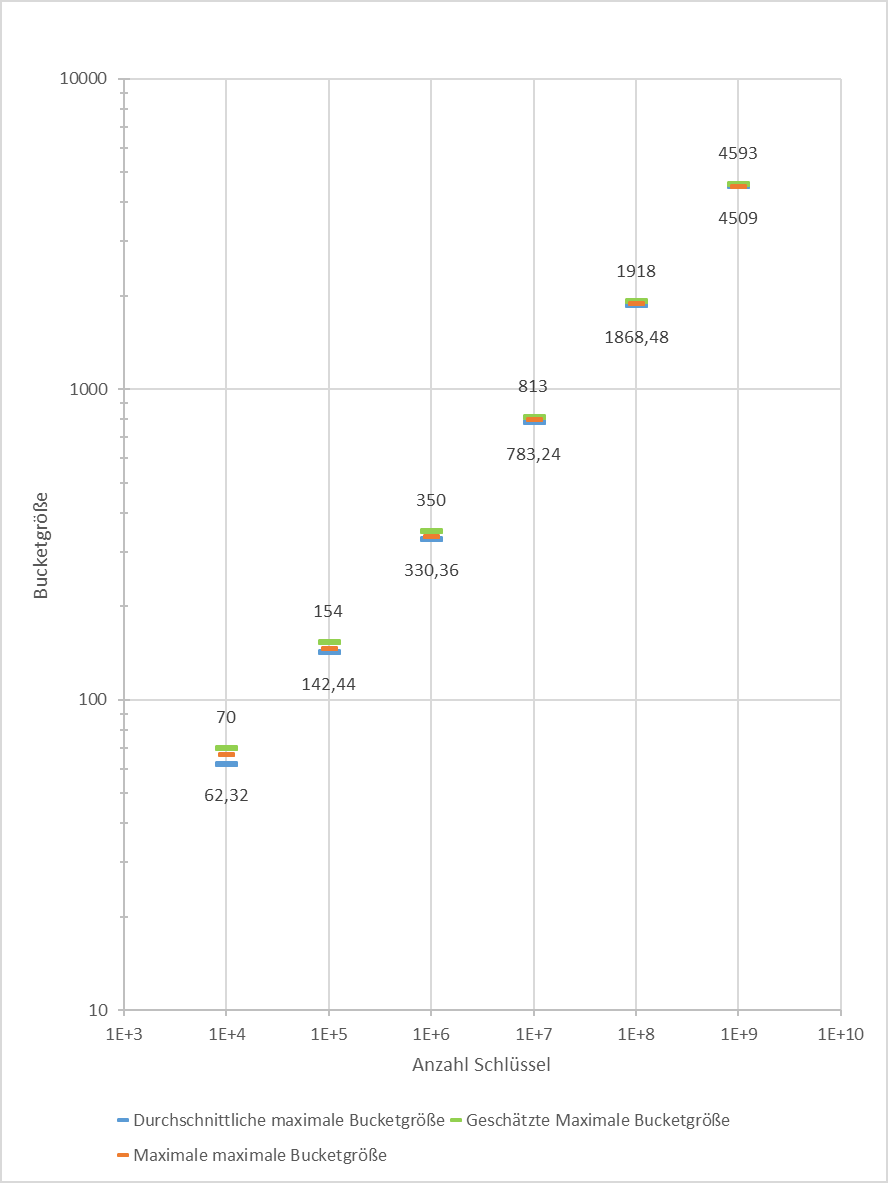
\includegraphics[width=\textwidth]{diagrams/TatsaechlicheUndGeschaetzteMaximaleBucketgroesse.png}
\caption{Tatsächliche und geschätzte maximale Bucketgröße in Abhängigkeit von $n$}
\label{img:tatsaechlicheUndGeschaetzteMaximaleBucketgroesse}
\end{figure}

In Abb. \ref{img:tatsaechlicheUndGeschaetzteMaximaleBucketgroesse} wird für gegebene $n$ unter Verwendung dieser Abschätzung die geschätzte mit den in den Testläufen tatsächlich aufgetretenen maximalen Bucketgrößen verglichen.
Während die absolute Abweichung der geschätzten von der durchschnittlichen maximalen Bucketgröße für größere Schlüsselmengen zunimmt, sinkt die prozentuale Abweichung jedoch kontinuierlich:

\begin{table}[H]
\centering
\begin{tabular}{|c|c|c|c|c|c|c|}
\hline 
Anzahl Schlüssel & $10^4$ & $10^5$ & $10^6$ & $10^7$ & $10^8$ & $10^9$ \\ 
\hline 
Absolute Abweichung & $7,68$ & $11,56$ & $19,64$ & $29,76$ & $49,52$ & $84$ \\ 
\hline 
Prozentuale Abweichung & $12,32\%$ & $8,12\%$ & $5,94\%$ & $3,80\%$ & $2,65\%$ & $1,86\%$ \\ 
\hline 
\end{tabular}
\caption{}
\end{table}
Für $n\geq 10^6$ ist der geschätzte Wert also tatsächlich relativ nah am tatsächlichen Wert.

Damit können wir die Abschätzung zur Bestimmung der Anzahl von Buckets, die den Gesamtspeicherplatz zu minimieren versucht, verwenden.

\begin{figure}[tbhp]
\centering
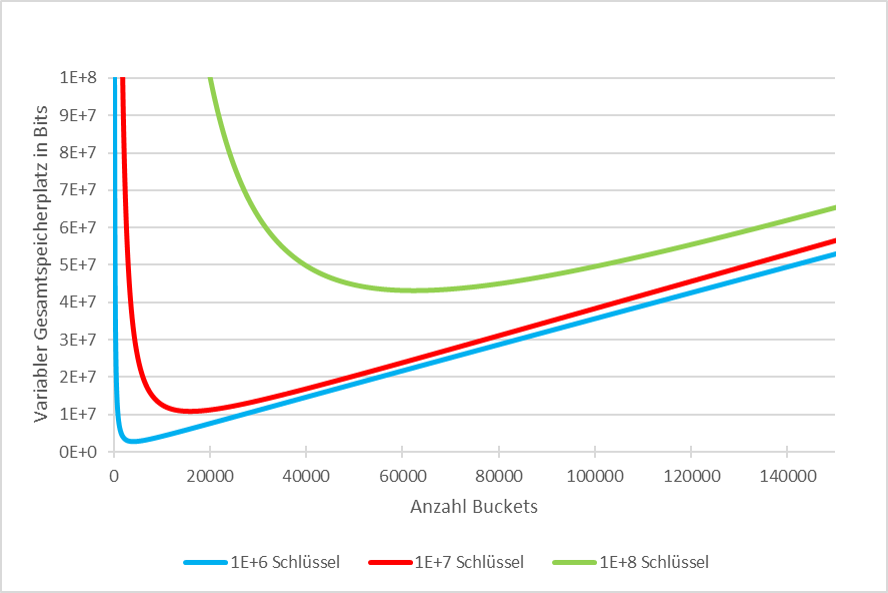
\includegraphics[width=0.9\textwidth]{diagrams/MinSizeZielfunktion.png}
\caption{Die zu minimierende Funktion (siehe Abschnitt \ref{sec:speicherplatz})}
\label{img:minSizeZielfunktion}
\end{figure}

In Abb. \ref{img:minSizeZielfunktion} wird der Anteil des Gesamtspeicherplatzes dargestellt, der von $m$ und $\hat{n}$ (mit der Abschätzung also von $n$ und $m$) abhängt.
Wie leicht zu sehen ist, ist die gesuchte Bucketanzahl $m$, die den Gesamtspeicherplatz minimiert, für $1\leq m\leq n$ eindeutig bestimmt.

\begin{figure}[tbhp]
\centering
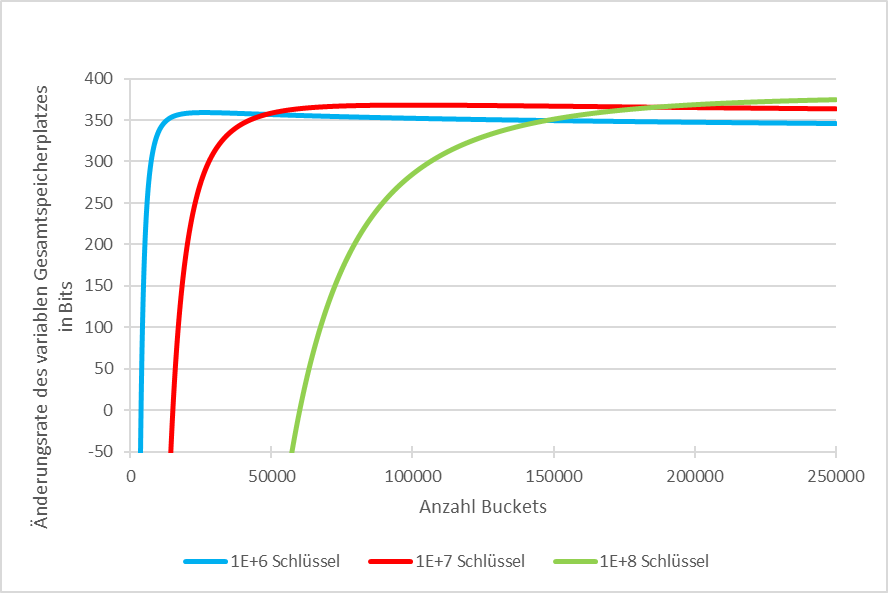
\includegraphics[width=0.9\textwidth]{diagrams/MinSizeZielfunktionAbleitung.png}
\caption{Die erste Ableitung der zu minimierenden Funktion}
\label{img:minSizeZielfunktionAbleitung}
\end{figure}

Um diese zu finden, betrachten wir die erste Ableitung der dargestellten Funktionen (siehe Abb. \ref{img:minSizeZielfunktionAbleitung}).
Mittels Bisektion (beginnend bei $m_{\min}=1$ mit negativem Funktionswert und $m_{\max}=n$ mit positivem Funktionswert der ersten Ableitung) kann somit in $\lceil\log n\rceil$ Schritten dasjenige $m$ gefunden werden, das der Nullstelle der Ableitung und somit dem Minimum der ursprünglichen Funktion am nächsten kommt.
Auch für $n=10^9$ sind dies nur $30$ Iterationen, in denen insgesamt $31$ Funktionswerte der ersten Ableitung berechnet werden müssen.


\section{Anzahl Buckets und durchschnittliche maximale Bucketgröße}
\label{sec:avgMaxBucketgroesse}

\begin{figure}[tbhp]
\centering
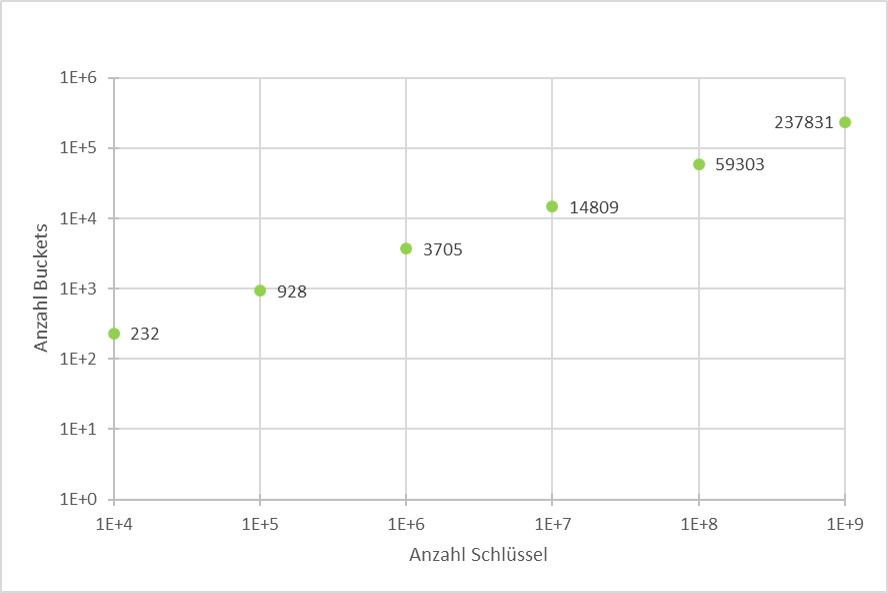
\includegraphics[width=0.9\textwidth]{diagrams/AnzahlBuckets.png}
\caption{Die berechneten Bucketanzahlen in Abhängigkeit von $n$}
\label{img:AnzahlBuckets}
\end{figure}
\begin{figure}[tbhp]
\centering
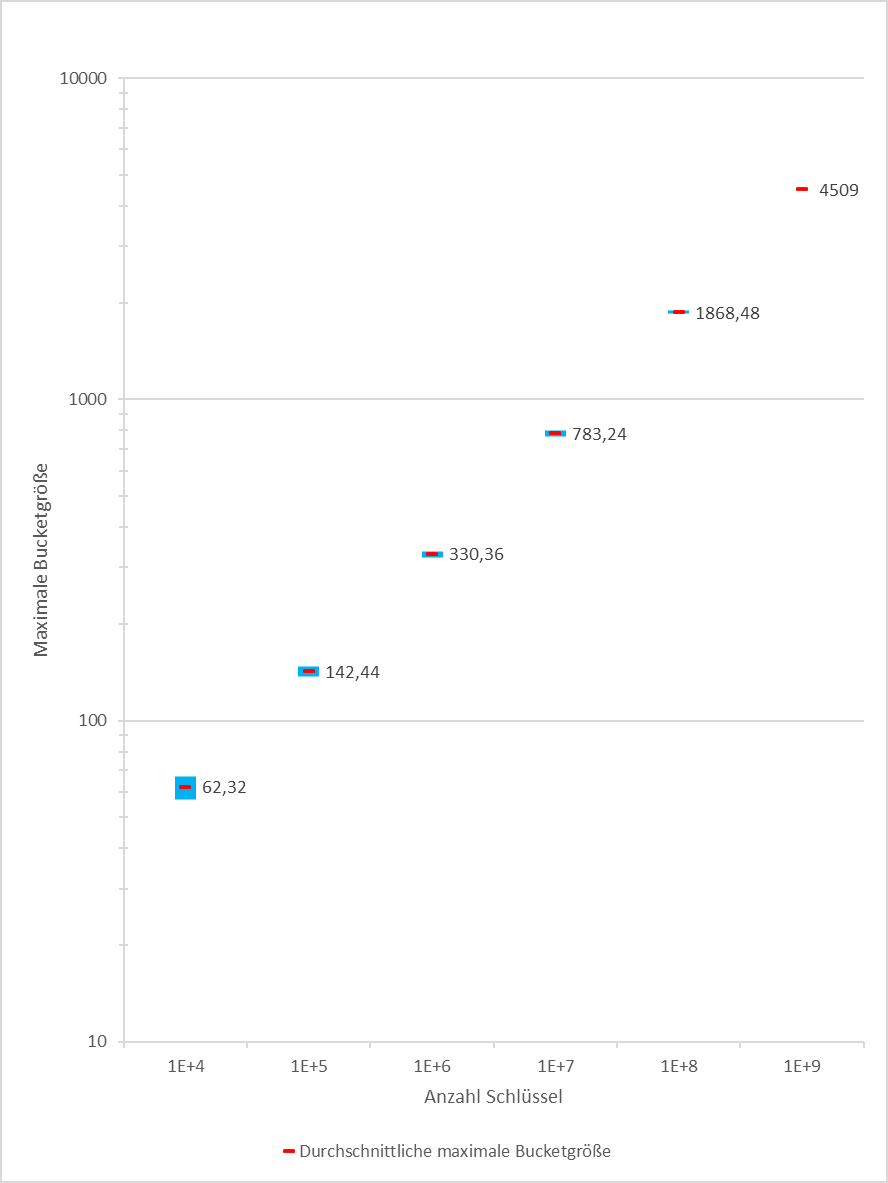
\includegraphics[width=\textwidth]{diagrams/MaximaleBucketgroesse.png} 
\caption{Die tatsächlich verwendeten maximalen Bucketgrößen in Abhängigkeit von $n$}
\label{img:MaximaleBucketgroesse}
\end{figure}
Unter Verwendung der in Abschnitt \ref{sec:schaetzungBucketgroesse} dargestellten Abschätzung ergaben sich in den Testläufen die in Abb. \ref{img:AnzahlBuckets} dargestellten Bucketanzahlen und die in Abb. \ref{img:MaximaleBucketgroesse} dargestellten zugehörigen tatsächlich aufgetretenen maximalen Bucketgrößen.
Während sowohl die Anzahl der Buckets als auch die durchschnittliche maximale Bucketgröße in etwa linear anwachsen (was ausschlaggebend für das Wachstum des Gesamtspeicherplatzes ist, siehe Abschnitt \ref{sec:speicherplatzOverhead}), verringert sich die relative Abweichung von der durchschnittlichen maximalen Bucketgröße bei steigender Schlüsselzahl kontinuierlich.
\pagebreak
\section{Durchschnittlicher Gesamtspeicherplatz und Split-and-Share-Overhead}
\label{sec:speicherplatzOverhead}

\begin{figure}[tbhp]
\centering
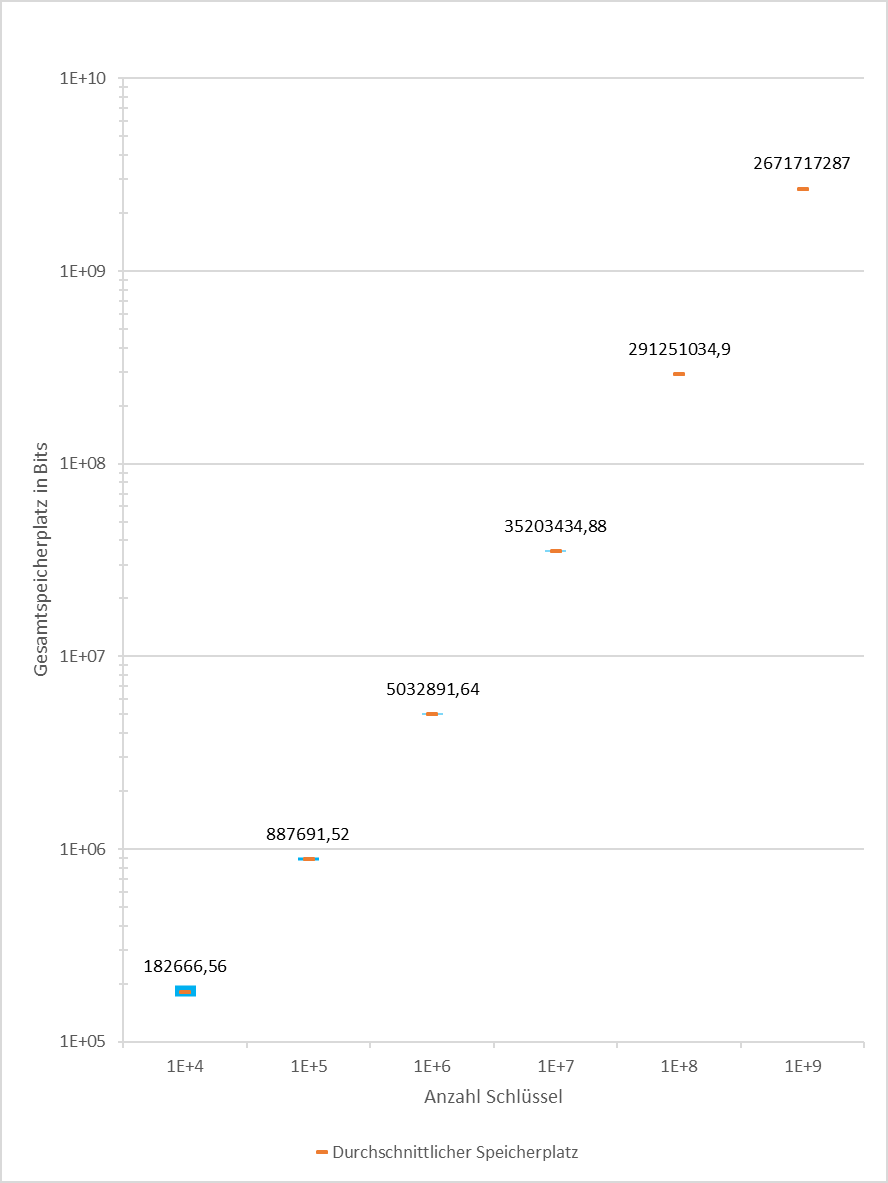
\includegraphics[width=\textwidth]{diagrams/Speicherplatz.png} 
\caption{Der Gesamtspeicherplatz in Bits in Abhängigkeit von $n$}
\label{img:Speicherplatz}
\end{figure}
In Abb. \ref{img:Speicherplatz} erkennen wir, dass der Gesamtspeicherplatz in etwa linear in der Größe der Schlüsselmenge wächst.
Dies liegt insbesondere an dem ebenfalls linearen Wachstum der Anzahl der Buckets und der durchschnittlichen maximalen Bucketgröße, was in Abschnitt \ref{sec:avgMaxBucketgroesse} beobachtet wurde.
Ebenso deckt sich dieses Ergebnis mit den theoretischen Überlegungen in \cite{Botelho2013108}.
\begin{figure}[tbhp]
\centering
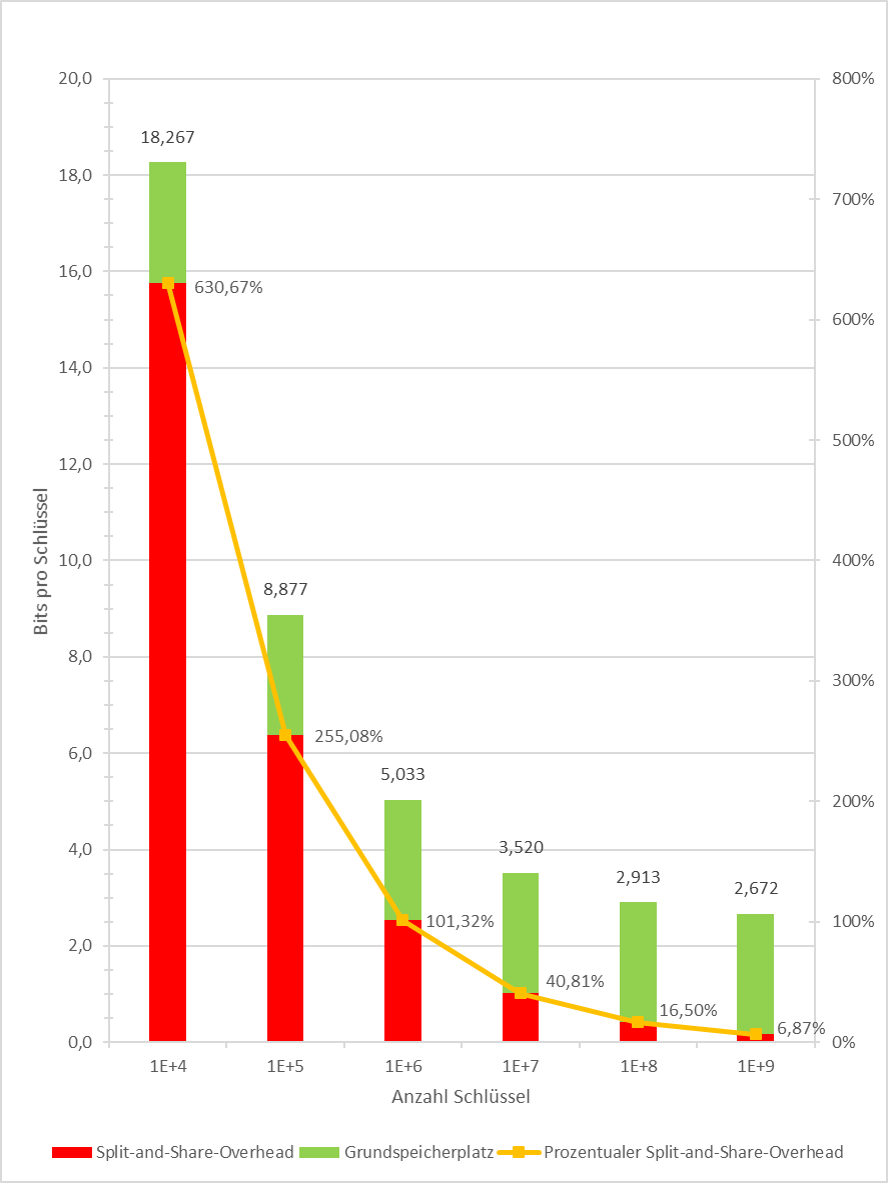
\includegraphics[width=0.95\textwidth]{diagrams/SplitAndShareOverhead.png} 
\caption{Die Anzahl der Bits pro Schlüssel sowie der prozentuale Anteil des Overheads in Abhängigkeit von $n$}
\label{img:SplitAndShareOverhead}
\end{figure}
Andererseits sinkt der relative Speicherplatz pro Schlüssel antiproportional zur Größe der Schlüsselmenge.
In Abb. \ref{img:SplitAndShareOverhead} sehen wir insbesondere, dass der zusätzlich zu den (auch ohne Verwendung des Split-and-Share-Verfahrens notwendigen) $2,5$ Bit pro Schlüssel entstehende Overhead ab $10^7$ Schlüsseln mit fast $40\%$ und insbesondere bereits für $10^8$ Schlüsseln mit $16,5\%$ erfreulich gering ist.

\section{Durchschnittlicher Overhead durch ``schlechte'' Zufallszahlen}
\label{sec:overheadZufallszahlen}

\begin{figure}[tbhp]
\centering
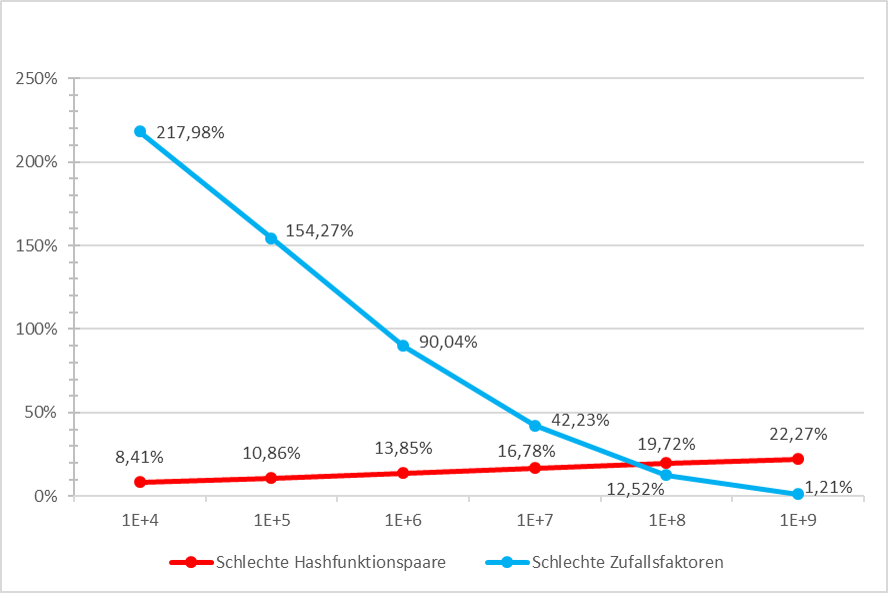
\includegraphics[width=\textwidth]{diagrams/OverheadZufallszahlen.png} 
\caption{Der Overhead durch Wahl ungünstiger Zufallszahlen in Abhängigkeit von $n$}
\label{img:OverheadZufallszahlen}
\end{figure}
An einigen Stellen bei der Konstruktion der perfekten Hashfunktion sind wir auf die Wahl zufälliger Zahlen angewiesen, die anschließend gute Eigenschaften erfüllen müssen.

Während die Wahl der Splitfunktion $h_{\text{split}}$ in sämtlichen Testläufen sofort erfolgreich war (d.h. die einzelnen Buckets wurden nicht zu groß), kam es - wie in Abb. \ref{img:OverheadZufallszahlen} zu sehen - gelegentlich vor, dass ein zufälliges Paar 1-universeller Hashfunktionen nicht gut war.
Allerdings beschränkte sich dies selbst bei größeren Schlüsselmengen nur auf einen geringen (aber wie zu erwarten wachsenden) Anteil.

Ebenso erwies sich die Einführung der Zufallsfaktoren $s_i$ als Ergänzung zu den Zufallstabellen als äußerst sinnvoll.
Während in keinem der Durchläufe neue Tabellen erzeugt werden mussten, zeigte sich besonders für kleine Schlüsselmengen eine erhöhte Notwendigkeit, einen anderen Zufallsfaktor zu erzeugen, da die damit in Abschnitt \ref{sec:perfekteHashfunktionProBucket} beschriebene erzeugte Hashfunktion nicht injektiv war.
Da der Anteil wiederholter Erzeugungen von Zufallszahlen sogar noch im Bereich von $10^6$ bis $10^8$ Schlüsseln von knapp $90\%$ auf $12,52\%$ fällt, hätte dies katastrophale Folgen auf die Laufzeit gehabt, wenn stattdessen immer wieder neue Zufallstabellen hätten erzeugt werden müssen, die wiederum für sämtliche Buckets eine gute Eigenschaft besitzen müssen.

\section{Durchschnittliche Konstruktionszeit}
\label{sec:konstruktionszeit}

\begin{figure}[tbhp]
\centering
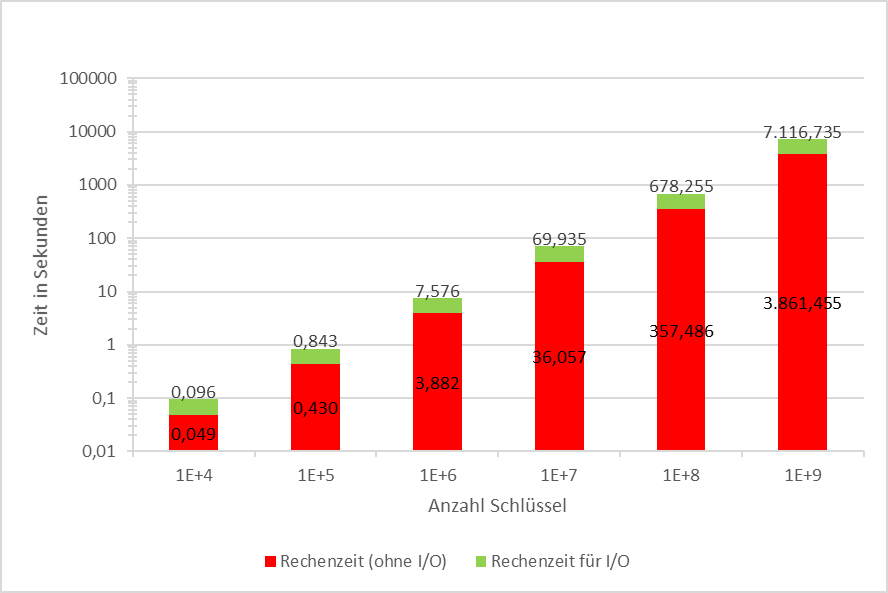
\includegraphics[width=0.9\textwidth]{diagrams/Konstruktionszeit.png} 
\caption{Die durchschnittliche Konstruktionszeit sowie der Anteil der I/O-Operationen in Abhängigkeit von $n$}
\label{img:Konstruktionszeit}
\end{figure}
Die auf dem Testrechner erreichten Konstruktionszeiten liegen (trotz der Verwendung temporärer Dateien) für $n\leq 10^8$ in einem akzeptablen Rahmen.
Wie in Abb. \ref{img:Konstruktionszeit} zu sehen, wächst die Konstruktionszeit in etwa proportional mit der Größe der Schlüsselmenge.
Dies deckt sich also mit den theoretischen Überlegungen aus \cite{Botelho2013108}.
Ebenso kann man den doch relativ hohen Anteil der Zeit für die I/O-Operationen (fast $50\%$) erkennen.
Auf entsprechender Hardware, die auch für größere Schlüsselmengen nicht auf das Arbeiten mit temporären Dateien angewiesen ist, sollte sich dieser Anteil entsprechend deutlich reduzieren lassen.


\section{Durchschnittliche Auswertezeit}
\label{sec:auswertezeit}

\begin{figure}[tbhp]
\centering
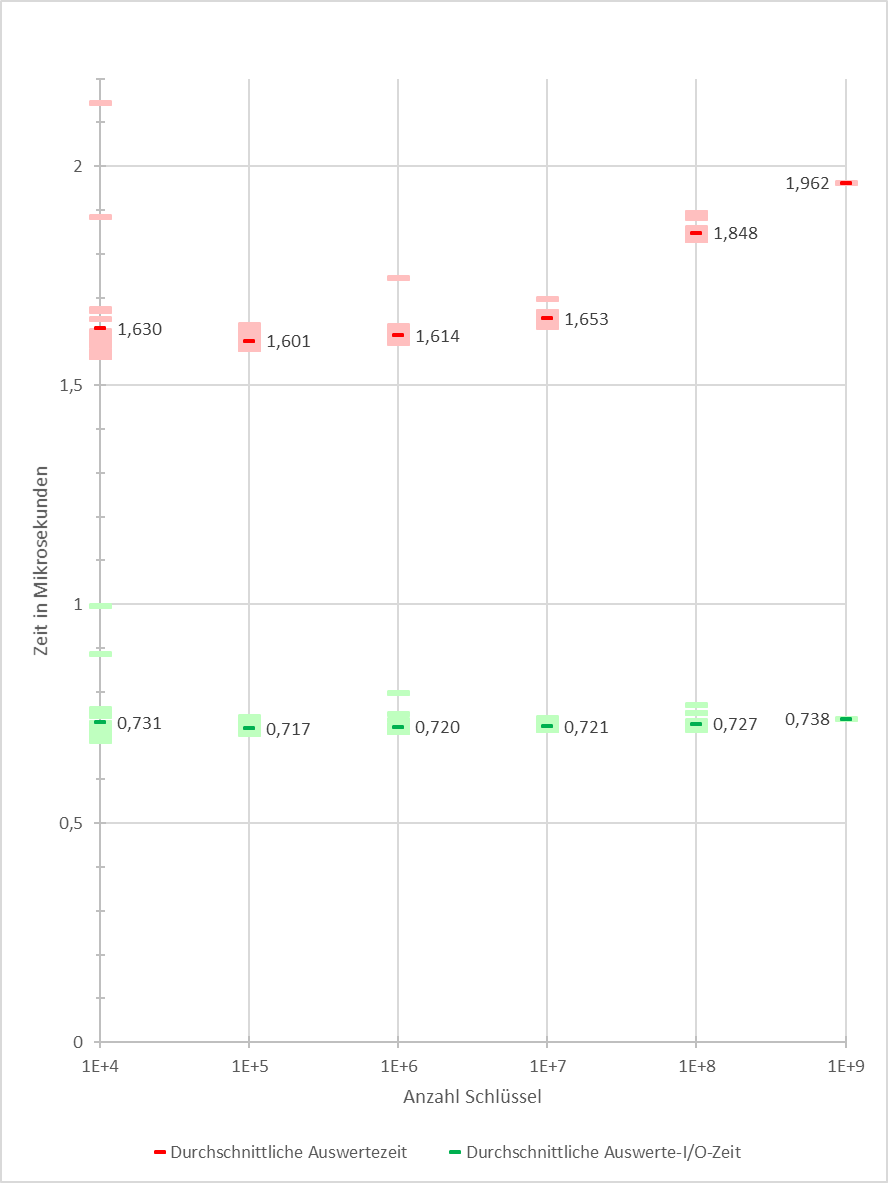
\includegraphics[width=\textwidth]{diagrams/Auswertezeit.png} 
\caption{Die durchschnittliche Auswertezeit pro Schlüssel in Abhängigkeit von $n$}
\label{img:Auswertezeit}
\end{figure}
Abschließend haben wir noch die benötigte Zeit zur Auswertung, d.h. Berechnung des Hashwertes für einen gegebenen Schlüssel, untersucht.
Im Einklang mit unserem Ziel blieb diese auch für große Schlüsselmengen im Wesentlichen konstant.
Abb. \ref{img:Auswertezeit} zeigt die pro Testlauf gemessenen durchschnittlichen Auswertezeiten und deren Mittelwerte.

\chapter{Fazit}
\label{cha:fazit}

Unsere Untersuchungen haben gezeigt, dass das ``Split-and-Share''-Verfahren zur Konstruktion perfekter Hashfunktionen auch für ``kleine'' Schlüsselmengen (zwischen $10^6$ und $10^8$ Schlüssel) sinnvoll sein kann.
Einerseits der nicht mehr zu große Overhead bzgl. des Gesamtspeicherplatzes (Abschnitt \ref{img:SplitAndShareOverhead}) und andererseits die hohen Erfolgsquoten und geringen Anzahlen wiederholter Erzeugungen von Zufallszahlen (Abschnitt \ref{img:OverheadZufallszahlen}) weisen das ``Split-and-Share''-Verfahren auch für diese Schlüsselmengen als geeignet aus.

Zum Schluss sei nochmals angemerkt, dass unsere Implementierung natürlich Spielraum zum Optimieren von Gesamtspeicherplatz (z.B. arithmetische Kodierung) und Konstruktions- sowie Auswertezeiten (z.B. effizientere Datenstrukturen und Algorithmen, z.B. für den Azyklizitätstest) lässt.

\cleardoublepage
\tocentry{Literaturverzeichnis}
\bibliography{literature}
\bibliographystyle{test}

\end{document}
